\chapter{Protocol of work so far}
\section{Rotated lines experiment}

\subsection{Introduction}
The goal of this task was to recreate example 2 from \citet{nessler}. In this example they fed a winner-take-all spiking neural network images with lines in different orientations on them. The network then clustered the images into ten groups depending on their orientation.

\subsection{Methods}
\paragraph{Input data}
The images used in this task were generated with a size of 29 x 29 pixel. Black lines going through the center of the image were drawn onto a white background. To simulate noise each pixel had a ten percent chance to have its color flipped. To ensure that all lines in the images have the same length regardless of their orientation a circular mask with a radius of 15 pixel was applied to the images. This recolored all pixel outside of the mask to white. During the training of the network these images were generated in uniformly distributed orientations for each training step. The random chosen orientation could lie between 0 and 359 degrees.  Two examples of such images can be seen in figure \ref{fig:angleImages}.

\begin{figure}
  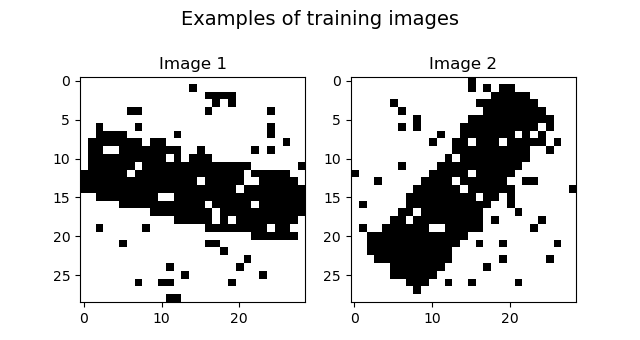
\includegraphics[width=\linewidth]{figures/angleNetwork/trainingImages.png}
  \caption{Two examples of the generated training data in this experiment.}
  \label{fig:angleImages}
\end{figure}

\paragraph{Neuron model}

As in \citet{nessler} the input neurons X are firing according to a poisson process with an average firing rate of 20 Hz when active and with 0 Hz when in an inactive state. The excitatory post synaptic potentials (EPSPs) $x_i(t)$ these neurons produce can be seen in figure \ref{fig:XSpike}.

\begin{figure}
  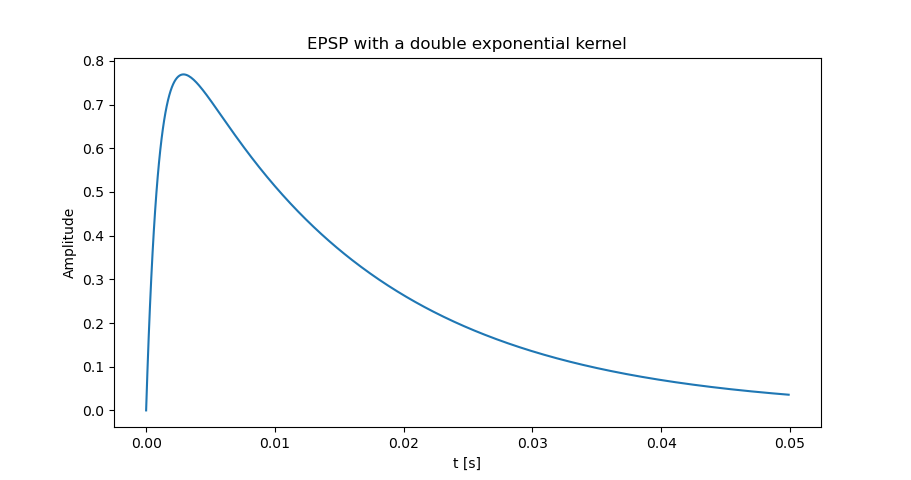
\includegraphics[width=\linewidth]{figures/XSpike.png}
  \caption{Form of an excitatory post synaptic potential generated by a X neuron over time. A double exponential kernel was used to generate this signal. These signals are fed to the next layer of the network. }
  \label{fig:XSpike}
\end{figure}

The firing rate of an output neuron $Y_k$ depends exponentially on its membrane potential $U_k$ and the inhibitory signal $I_{inh}$ it receives. The membrane potential of an Y neuron depends on the EPSPs of all X neurons. This can be seen in equation \ref{eqn:rk}. The chance of an individual Y neuron to fire within a time step $\delta t$ is given in equation \ref{eqn:rkdt}.

\begin{equation}
\label{eqn:rk}
r_k(t) = e^{u_k(t) - I(t)}
\end{equation}

\begin{equation}
\label{eqn:rkdt}
r_k(t) \cdot \delta t
\end{equation}

\paragraph{Network architecture}
Each pixel of an input image was connected to two neurons. The first of these neurons is in an active state when the pixel is black and in an inactive state otherwise. The second neuron expresses the opposite behaviour. As a consequence the network needs 1682 ($29 \cdot 29 \cdot 2$) excitatory input neurons $x_1,...,x_n$. These X neurons are then fully connected to ten excitatory output neurons $y_1,...,y_k$. This means that that every input neuron $x_i$ is connected to each output neuron $y_k$. The membrane potential $U_k$ of each Y neuron is calculated by multiplying the EPSP of each X neuron times the weight of the connection between the X and Y neuron. 
\begin{equation}
\label{eqn:uk}
U_k(t) = \sum_{i=1}^n w_{ki} \cdot x_i(t)
\end{equation}
In \citet{nessler} each Y neuron also had an intrinsic excitability $w_{k0}$ which was learned for each neuron. For this experiment however it was omitted, as each orientation of input images was equally likely, thus the intrinsic excitability of each Y neuron would end up being the same.

The Y neurons are modelled in a winner-takes-all (WTA) circuit. This means that whenever one Y neuron spikes, a lateral inhibitory signal is fed to all Y neurons, thus preventing the further activation of all output neurons for 5 ms. After the training of the network each Y neuron should be active for lines in an 18° area. 


\paragraph{Inhibition}
The inhibition signal was chosen to depend on the current membrane potential of the Y neurons. According to \citet{nessler} the overall firing rate of the Y neurons is:
\begin{equation}
\label{eqn:R}
R(t) = \sum_{k=1}^K e^{U_k(t) - I(t)}
\end{equation}
Solving this equation for I(t):
\begin{equation}
\label{}
R(t) = \frac{ \sum_{k=1}^K e^{U_k(t)}}{e^{I(t)}}
\end{equation}
\begin{equation}
\label{}
e^{I(t)} = \frac{\sum_{k=1}^K e^{U_k(t)}}{R(t)}
\end{equation}
\begin{equation}
\label{}
I(t) = \ln{ \frac{ \sum_{k=1}^K e^{U_k(t)}}{R(t)}}
\end{equation}
\begin{equation}
\label{eqn:I(t)}
I(t) =  - \ln{R(t)} + \ln{  \sum_{k=1}^K e^{U_k(t)}}
\end{equation}
When implementing the inhibition the $- \ln{R(t)}$ term of equation \ref{eqn:I(t)} was overlooked, that means it was assumed to be zero. Because of that R(t) equals 1 when the inhibition is active. This error was not detected at first, as the chance that a Y neuron fires within a time step of 1 ms with active inhibition is 1/1000 due to that oversight.

Whenever a Y neuron produces a spike the inhibition signal I(t) is subtracted from the membrane potential Uk(t) of every Y neuron. This happens for the duration of $\sigma_{inh} = 5 ms$. Thus follows:

\begin{equation}
\label{eqn:iinh}
I(t) = \begin{dcases*} \ln ( \sum_{i=1}^k e^{U_k} ) & if any $y_k$ fired in $ [t^f, t^f  + \sigma_{inh}] $ \\
0 & \text{if any $y_k$ did not fire in $ [t^f, t^f + \sigma_{inh}] $ } \end{dcases*}\end{equation}

\paragraph{Spike time dependent plasticity}
The weights $w_{ki}$ between neurons $x_i$ and $y_k$ are updated whenever a Y neuron fires. The time window $\sigma$ was set as 10 ms according to \citet{nessler}. The other parameters c and learning rate $\lambda$ were determined via grid search (see results).
\begin{equation}
\label{deltawki}
\Delta w_{ki} = \begin{dcases*} \lambda \cdot (ce^{-w_{ki}} - 1) & if $x_{i}$ fired in $ [t^f - \sigma, t^f] $ \\
\lambda \cdot (-1) & \text{if $ x_i $ did not fire in $ [t^f - \sigma, t^f] $ } \end{dcases*}
\end{equation}
\begin{tabbing}
\phantom{$c\ $}\= \kill
where:\> \\
$\lambda$\> ... learning rate \\
c\> ... shifts weights values \\
$t^f$\> ... time of y spike \\
$\sigma$ ... time window in which X spikes are considered as "before" Y spike
\end{tabbing}


\subsection{Results}
